%% abtex2-modelo-relatorio-tecnico.tex, v-1.7.1 laurocesar
%% Copyright 2012-2013 by abnTeX2 group at http://abntex2.googlecode.com/ 
%%
%% This work may be distributed and/or modified under the
%% conditions of the LaTeX Project Public License, either version 1.3
%% of this license or (at your option) any later version.
%% The latest version of this license is in
%%   http://www.latex-project.org/lppl.txt
%% and version 1.3 or later is part of all distributions of LaTeX
%% version 2005/12/01 or later.
%%
%% This work has the LPPL maintenance status `maintained'.
%% 
%% The Current Maintainer of this work is the abnTeX2 team, led
%% by Lauro César Araujo. Further information are available on 
%% http://abntex2.googlecode.com/
%%
%% This work consists of the files abntex2-modelo-relatorio-tecnico.tex,
%% abntex2-modelo-include-comandos and abntex2-modelo-references.bib
%%

% ------------------------------------------------------------------------
% ------------------------------------------------------------------------
% abnTeX2: Modelo de Relatório Técnico/Acadêmico em conformidade com 
% ABNT NBR 10719:2011 Informação e documentação - Relatório técnico e/ou
% científico - Apresentação
% ------------------------------------------------------------------------ 
% ------------------------------------------------------------------------

% Alterado por Rodrigo Campiolo para apresentação de relatórios na disciplina
% de Redes de Computadores II do Bacharelado em Ciência da Computação da UTFPR-CM.


\documentclass[
	% -- opções da classe memoir --
	12pt,				% tamanho da fonte
	%openright,			% capítulos começam em pág ímpar (insere página vazia caso preciso)
	oneside,   	        % para impressão em verso e anverso use twoside. Oposto a oneside
	a4paper,			% tamanho do papel. 
	% -- opções da classe abntex2 --
	chapter=TITLE,		% títulos de capítulos convertidos em letras maiúsculas
	section=TITLE,		% títulos de seções convertidos em letras maiúsculas
	subsection=TITLE,	% títulos de subseções convertidos em letras maiúsculas
	subsubsection=TITLE,% títulos de subsubseções convertidos em letras maiúsculas
	% -- opções do pacote babel --
	english,			% idioma adicional para hifenização
	french,				% idioma adicional para hifenização
	spanish,			% idioma adicional para hifenização
	brazil,				% o último idioma é o principal do documento
	]{pacotes/abntex2}


% ---
% PACOTES
% ---

% Pacotes fundamentais
% ---
\usepackage{cmap} % Mapear caracteres especiais no PDF
\usepackage{lmodern} % Usa a fonte Latin Modern
\usepackage[T1]{fontenc} % Selecao de codigos de fonte.
\usepackage[utf8]{inputenc} % Codificacao do documento (conversão automática dos acentos)
\usepackage{indentfirst} % Indenta o primeiro parágrafo de cada seção.
\usepackage{color} % Controle das cores
\usepackage{graphicx} % Inclusão de gráficos

% ---
\usepackage[utf8]{inputenc}

\usepackage{float}
% ---
% Pacotes adicionais, usados no anexo do modelo de folha de identificação
% ---
\usepackage{multicol}
\usepackage{multirow}
% ---

% ---
% Pacotes adicionais, usados apenas no âmbito do Modelo Canônico do abnteX2
% ---
\usepackage{lipsum} % para geração de dummy text
% ---

% ---
% Pacotes de citações
% ---
\usepackage[brazilian,hyperpageref]{backref} % Paginas com as citações na bibl
\usepackage[alf]{abntex2cite} % Citações padrão ABNT
\usepackage{comment}
% ---

% CONFIGURAÇÕES DE PACOTES
% ---

% % ---
% ---
% Configurações do pacote backref
% Usado sem a opção hyperpageref de backref
\renewcommand{\backrefpagesname}{Citado na(s) página(s):~}
% Texto padrão antes do número das páginas
\renewcommand{\backref}{}
% Define os textos da citação
\renewcommand*{\backrefalt}[4]{
	\ifcase #1 %
		Nenhuma citação no texto.%
	\or
		Citado na página #2.%
	\else
		Citado #1 vezes nas páginas #2.%
	\fi}%
% ---

%%%%%%%%%%%%%%%%%%%%%% SOBRE O TRABALHO %%%%%%%%%%%%%%%%%%%%%%%%%%%%%%%
%A partir do projeto de Extensão, no qual pretende resolver o problema de obesidade, fazer a imersão no tema.

%Escolher e executar 1 das técnicas de imersão preliminar + das 1 técnicas de imersão de profundidade.


%IMERSÃO PRELIMINAR
%Reenquadramento
%Pesquisa Exploratória
%Pesquisa Desk


%IMERSÃO EM PROFUNDIDADE
%Entrevistas
%Cadernos de sensibilização
%Sessão generativa
%Um dia na vida
%Sombra

%Escolhemos: Pesquisa Desk (imersão preliminar) e Um dia na vida (Imersão em profundidade)
 
%Entregar em formato de relatório nas normas da ABNT.
%%%%%%%%%%%%%%%%%%%%%%%%%%%%%%%%%%%%%%%%%%%%%%%%%%%%%%%%%%%%%%%%%%%%%%%%%%%%%%%%%%%%%%%%%%%%

% ---
% Informações de dados para CAPA e FOLHA DE ROSTO
% ---
\titulo{Trabalho Bimestral de Gestão de Equipes e Projetos}
\autor{Igor Ortega Carmona | RA: 00236524 \\ Eduardo Fagotti | RA: 00222820 \\ Kaully Hayashi | RA: 00219066 \\ Vitor Agostini | RA: 00241431 }
\local{Cianorte}
\data{Abril / 2023}
\instituicao{%
  UNIPAR - CIANORTE
  \par
  Tecnologia em Análise e Desenvolvimento de Sistemas (ADS)
}
\tipotrabalho{Relatório técnico}
% O preambulo deve conter o tipo do trabalho, o objetivo, 
% o nome da instituição e a área de concentração 
\preambulo{Trabalho bimestral sobre as técnicas de imersão preliminar e em profundidade aplicada solicitado pelo professor Dr.Thiago Martins para a matéria de \textit{Gestão de Equipes e Projetos} grade do curso de \textit{Análise e Desenvolvimento de Sistemas}. }
% ---

% ---
% Configurações de aparência do PDF final

% alterando o aspecto da cor azul
\definecolor{blue}{RGB}{41,5,195}

% informações do PDF
\makeatletter
\hypersetup{
     	%pagebackref=true,
		pdftitle={\@title}, 
		pdfauthor={\@author},
    	pdfsubject={\imprimirpreambulo},
	    pdfcreator={LaTeX with abnTeX2},
		pdfkeywords={abnt}{latex}{abntex}{abntex2}{relatório técnico}, 
		colorlinks=true,       		% false: boxed links; true: colored links
    	linkcolor=blue,          	% color of internal links
    	citecolor=blue,        		% color of links to bibliography
    	filecolor=magenta,      		% color of file links
		urlcolor=blue,
		bookmarksdepth=4
}
\makeatother
% --- 

% --- 
% Espaçamentos entre linhas e parágrafos 
% --- 

% O tamanho do parágrafo é dado por:
\setlength{\parindent}{1.3cm}

% Controle do espaçamento entre um parágrafo e outro:
\setlength{\parskip}{0.2cm}  % tente também \onelineskip

% ---
% compila o indice
% ---
\makeindex
% ---

% Omite a numeração de capítulos
\renewcommand*\thesection{\arabic{section}}



% ----
% Início do documento
% ----
\begin{document}

% Retira espaço extra obsoleto entre as frases.
\frenchspacing 

% ----------------------------------------------------------
% ELEMENTOS PRÉ-TEXTUAIS
% ----------------------------------------------------------
% \pretextual

% ---
% Capa
% ---
%\imprimircapa
% ---

% ---
% Folha de rosto
% (o * indica que haverá a ficha bibliográfica)
% ---
\imprimirfolhaderosto
% ---


% ---
% RESUMO
% ---

% resumo na língua vernácula (obrigatório)
\begin{resumo}
 
 Este trabalho bimestral aborda as técnicas de imersão preliminar e em profundidade de forma aplicada ao contexto real de um estudo de projeto. Foi realizado um acompanhamento de rotina diário de uma pessoa afim de validar a etapa \textit{"Um dia na vida"} do \textit{Design Thinking} e pesquisas aprofundadas sobre o tema \textbf{Obesidade}, na qual, é também o tema estudado pelo Projeto de Extensão da Universidade UNIPAR de Cianorte.

 \vspace{\onelineskip}
    
 \noindent
 \textbf{Palavras-chave}: Obesidade, Imersão preliminar, Imersão em profundidade, Gestão de Projetos.
\end{resumo}
% ---
\begin{resumo}[Abstract]
  \begin{otherlanguage*}{english}
    This bimonthly assignment addresses preliminary and in-depth immersion techniques applied to the real context of a design study. Daily routine monitoring of a person was conducted to validate the \textit{"A day in the life"} stage of \textit{Design Thinking}, as well as in-depth research on the topic of \textbf{Obesity}, which is also the subject studied by the Extension Project of UNIPAR University in Cianorte.
    
    \vspace{\onelineskip}
    
    \noindent\textbf{Keywords}: Obesity, Preliminary Immersion, In-depth Immersion, Project Management.
  \end{otherlanguage*}
\end{resumo}
% ---
% inserir lista de ilustrações
% ---
%\pdfbookmark[0]{\listfigurename}{lof}
%\listoffigures*
%\cleardoublepage
% ---

% ---
% inserir lista de tabelas
% ---
%\pdfbookmark[0]{\listtablename}{lot}
%\listoftables*
%\cleardoublepage
% ---

% ---
% inserir lista de abreviaturas e siglas
% ---
\begin{siglas}
  \item[CDC] Centers for Disease Control
  \item[NHANES] National Health and Nutrition Examination Survey
  \item[EUA] United States of American
  \item[IMC] Índice de Massa Corpórea 
\end{siglas}
% ---

% ---
% inserir o sumario
% ---
\pdfbookmark[0]{\contentsname}{toc}
\tableofcontents*
\cleardoublepage
% ---

% ----------------------------------------------------------
% ELEMENTOS TEXTUAIS
% ----------------------------------------------------------

%------------------------------------------------------------------------%
%% PARA FAZER CITAÇÕES
  %  \cite{kernel/Linux}.
%------------------------------------------------------------------------%


%------------------------------------------------------------------------%
%%LISTAGEM DE ITENS

%\begin{itemize}
%    \item \textbf{Virtual Box 6.1:} TEXTO
%\end{itemize}
%\begin{itemize}
%    \item \textbf{Distribuição Linux GNU/Debian 11.4:} TEXTO
%\end{itemize}
%\begin{itemize}
%    \item \textbf{kernel Linux 5.19.2:} TEXTO
%\end{itemize}
%------------------------------------------------------------------------%


%-------------------------------------------------------------------------%
  %% COLOCAR SITES
  
 % \url{https://www.debian.org/download}.
%-------------------------------------------------------------------------%
 
 
%-------------------------------------------------------------------------%    
%%%% COLOCAR FIGURAS %%%%

 %   \begin{figure}[H]
  %\centering
  %\includegraphics[scale=0.8]{figuras/vm.png}
  %\caption{Configurações inicias da máquina}
  %\label{fig:partições}
%\end{figure}
%------------------------------------------------------------------------%

\textual

\makeatletter
\renewcommand{\chapter}{\@gobbletwo}
\makeatother

\section{\textbf{Imersão preliminar - Pesquisa Desk}}
\label{sec:pesquisadesk}

O \textit{Centers for Disease Control and Prevention (CDC)}, conduziu uma pesquisa com o objetivo de avaliar a prevalência de obesidade e obesidade grave entre adultos nos Estados Unidos. 

A pesquisa utilizou o \textit{National Health and Nutrition Examination Survey (NHANES)} \cite{content}, que é uma amostra nacionalmente representativa da população americana, para medir o índice de massa corporal (IMC) dos participantes e categorizá-los como tendo obesidade (IMC de 30 ou mais) ou obesidade grave (IMC de 40 ou mais). 

A pesquisa revelou que a prevalência de obesidade entre adultos nos EUA era de 42,4\%, com 9,2\% dos adultos tendo obesidade grave. As taxas de obesidade foram mais altas entre adultos com idade entre 40-59 anos e com 60 anos ou mais, e mais baixas entre adultos com idade entre 20-39 anos.

%%%% COLOCAR FIGURAS %%%%
\begin{figure}[H]
  \centering
  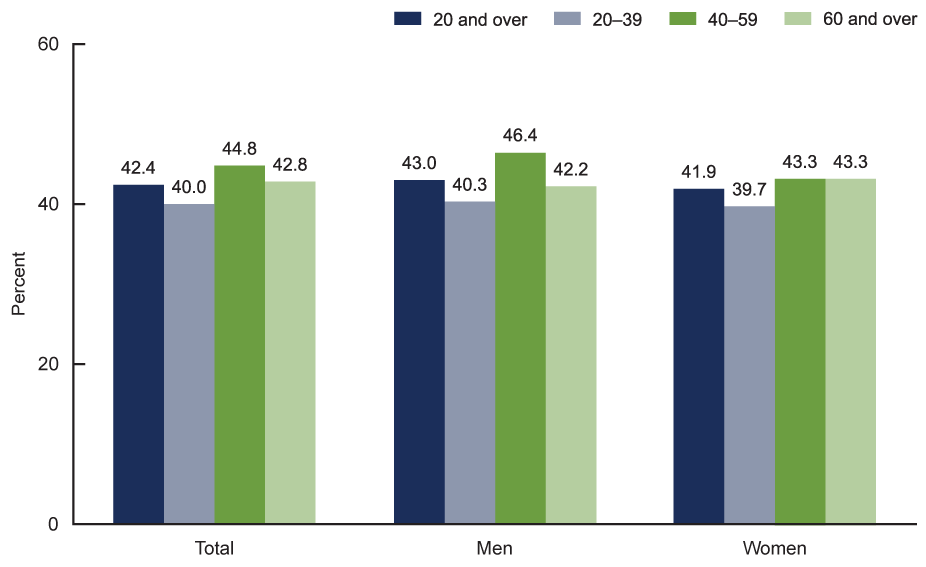
\includegraphics[height=9cm]{Figuras/fig-gestao.png}
  \caption{Prevalência de obesidade entre adultos com 20 anos ou mais, por sexo e idade: Estados Unidos, 2017-2018. 
  As estimativas para adultos com 20 anos ou mais foram ajustadas por idade pelo método direto para a população do censo dos Estados Unidos de 2000, utilizando os grupos etários de 20-39, 40-59 e 60 anos ou mais. As estimativas brutas são de 42,5\% para o total, 43,0\% para homens e 42,1\% para mulheres.}
  \label{fig:tabela-prevalence}
\end{figure}
%------------------------------------------------------------------------%

Além disso, adultos negros não hispânicos e adultos hispânicos apresentaram taxas mais altas de obesidade do que adultos brancos não hispânicos. A pesquisa destaca a necessidade de intervenções contínuas de saúde pública para combater a epidemia de obesidade e suas consequências associadas à saúde.

\section{\textbf{Imersão em Profundidade - Um dia na vida de Pedro Henrique}}
\label{sec:imersaoprofunda}

Pedro Henrique, (descrição pessoal detalhada no \nameref{apend:pedrohenrique}) \cite{Pedro} tem 27 anos de idade e mede 1,75 de altura. Ele tem dois irmãos que também estão acima do peso. Pedro enfrenta dificuldades para levantar da cama devido ao excesso de peso, o que causa dores e limita seus movimentos. Ao escolher suas roupas, muitas vezes ele tem dificuldade em encontrar peças que se adequem ao seu tamanho, causando estresse e constrangimento.

Ao se locomover até o trabalho, Pedro enfrenta dificuldades em espaços públicos, como calçadas que não são adaptadas para pessoas com obesidade e corredores apertados em lojas, o que dificulta sua movimentação. Durante o trabalho, ele sente dores nas costas e nos joelhos, além de se cansar com mais facilidade devido ao excesso de peso.

A hora do almoço pode ser um momento delicado para Pedro, já que precisa controlar sua alimentação para controlar seu peso, o que muitas vezes causa ansiedade. Ele também relata que é vítima de bullying e discriminação por causa de sua aparência, o que torna o momento do almoço um desafio emocional.

Ao final do dia de trabalho, Pedro sente mais dificuldades para realizar atividades cotidianas, como ir ao supermercado ou praticar exercícios físicos, pois seu cansaço e desconforto físico prejudicam sua qualidade de vida e autoestima. Além disso, seu pai está afastado da família devido a brigas familiares, o que pode aumentar o estresse e a ansiedade dele.

Ao finalizar a experiência da Imersão, ele diz ter vontade de mudar vida adotando hábitos mais saudáveis, controlando sua alimentação e praticando exercícios físicos para perder peso e melhorar sua saúde e autoestima.

\newpage
% O comando \newpage indica ao LaTeX para que seja inserida uma nova página no documento.
% ----------------------------------------------------------
% ELEMENTOS PÓS-TEXTUAIS
% ----------------------------------------------------------
\postextual
% ----------------------------------------------------------
% Referências bibliográficas
% ----------------------------------------------------------
\renewcommand{\bibsection}{%
\section{\bibname}
\bibmark
%\ifnobibintoc\else
%\phantomsection
%\addcontentsline{toc}{section}{\bibname}
%\fi
\prebibhook}

\bibliography{abntex2-modelo-references}

% ----------------------------------------------------------
% Apêndices
% ----------------------------------------------------------

% ---
% Inicia os apêndices
% ---
 \begin{apendicesenv}
 
\section*{Apêndice A - Descrição de Pedro Henrique}
\label{apend:pedrohenrique}
\addcontentsline{toc}{section}{Apêndice A - Descrição de Pedro Henrique}
 
Pedro Henrique é um cientista da computação formado pela Universidade federal UTFPR de Campo Mourão, que cresceu em Cianorte apesar de ter nascido em São Paulo. Além de suas habilidades na área de tecnologia, ele mantém um blog onde compartilha conhecimento sobre o assunto. Ele é casado e tem um filho de três anos, chamado Miguel. Pedro Henrique é um ávido leitor e atualmente está lendo "Os Miseráveis", de Victor Hugo. Embora goste de esportes radicais, prefere assisti-los. Pedro Henrique é também um talentoso músico que toca piano e violão desde criança. Além disso, ele é poliglota e fala fluentemente inglês.
 
 \end{apendicesenv}
% % ---


% ----------------------------------------------------------
% Anexos
% ----------------------------------------------------------

% % ---
% % Inicia os anexos
% % ---
% \begin{anexosenv}

% % ---
% \section*{Anexo A - Nome do Anexo}
% \addcontentsline{toc}{section}{Anexo A - Nome do Anexo}
% % ---
% \end{anexosenv}


\end{document}
